% Modelo de Dissertação do Mestrado em Informática da PUC - Alterado para cumprir a normalização de 2011
%\documentclass[a4paper,brazil,ruledheader,normaltoc,capchap]{abnt}

% Para impressão frente e verso (normalização 2011)
\documentclass[a4paper,brazil,ruledheader,normaltoc,capchap,twoside,openany]{abnt_pucmg_utf8}
\usepackage{nomencl}
\makenomenclature

% Não esquecer das alterações no arquivo abnt.cls
% Se estiver usando o Kile no Ubuntu o arquivo fica armazenado em /usr/share/texmf/tex/latex/abntex.
% Comentar a linha 967 
% \vspace*{30pt}% - Linha comentada para reduzir o espaçamento entre o topo da página e o título \chapter
% Alterar a linha 1143
% \vspace*{-30pt} % - Parâmetro alterado de 30pt para -30pt para reduzir o espaçamento entre o top da página e o título do apêndice
% Alterar a linha 985
%\vspace*{-30pt}\par % - Parâmetro alterado de 0pt para -30pt para reduzir o espaçamento entre o top da página e o título \chapter*
% Alterar a linha 991
% Parâmetro alterado de 45pt para 30pt para reduzir o espaçamento entre o texto e o título \chapter*

% Não esquecer das alterações no arquivo acronym.sty
% Se estiver usando o Kile no Ubuntu o arquivo fica armazenado em /usr/share/texmf-texlive/tex/latex/acronym
% Alterar a linha 225
%\item[\protect\AC@hypertarget{#1}{\acsfont{\normalfont{#2}}} --] #3% - Inserir separador entre acrônimo/descrição e remover o negrito com o normalfont

% Pacote para definir explicitamente as margens das páginas
\usepackage[a4paper,left=3cm,right=2cm,top=3cm,bottom=2cm]{geometry}

%\usepackage{units}
% Utilize da seguinte forma \unit[78,6]{mA}

% Pacote para gerenciar siglas
\usepackage[printonlyused]{acronym}

\usepackage{booktabs}
\usepackage[table,xcdraw]{xcolor}

% Merge em duas células (linhas diferentes)
\usepackage{multirow}

% Pacote para citação e referências seguindo ABNT no sistema (AUTOR, Data)
%\usepackage[alf, bibjustif,abnt-emphasize=bf]{abntcite}
% MODIFICACAO BY DAVIDYSSON (TROQUEI O COMANDO ABAIXO DE ABNTCITE PARA ABNTEX2CITE)
%\usepackage[alf, abnt-emphasize=em, abnt-thesis-year=title]{abntcite}
\usepackage[alf, abnt-emphasize=em, abnt-thesis-year=title]{abntex2cite}
% @article An article from a journal or magazine 
% @inproceedings An article in a conference proceedings
% Força que o tipo de ênfase no nome do simpósio seja em caixa alta
\renewcommand{\emph}{\textsc}

% Pacote para múltiplos arquivos .bib
\usepackage{multibib}
%\newcites{pub}{Refer\^encias das publica\c{c}\~oes}

% Pacote de adequação do formato ABNT para normas da PUCMinas
\usepackage{abnt-PPGInf-PUCMG}
	
% Pacotes utilitários
\usepackage{graphicx}

% Pacote para fixar a figura no local desejado
\usepackage{float}

% Pacote para adicionar simbolos as informações de rodapé
\usepackage[symbol]{footmisc}

\usepackage[all]{xy}
%\usepackage[tight]{subfigure}	% Permite a criação de subfiguras
\usepackage{url,amsmath}	% Permite melhorias na codificação de fórmulas
%\usepackage{amsthm}		% Permite melhorias na escrita de teoremas
\usepackage{amssymb}		% Permite utlização de simbolos matemáticos avançados

\usepackage[portuguese, linesnumbered, ruled, vlined]{algorithm2e}
\usepackage{algorithmic} 	% para algoritmos
\usepackage{listings} 		% para importação de código-fonte

% Alterar o espaçamento da margem no algoritmo
\setlength{\algomargin}{1em}

\usepackage{setspace}

% Pacote para rotação de tabelas/figuras
\usepackage{rotating}

% Pacotes para criação de cronograma/tabela colorida
\usepackage{color}
\usepackage{array}
\usepackage{longtable}
\usepackage{colortbl}
%\definecolor{lightgray}{gray}{0.9}

\usepackage{paralist}

% Pacote para possibilitar o uso do setboolean para forçar formatos de página diferentes do padrão do documento
\usepackage{ifthen}

% Para inserir captions (nova normalização 2011)
\usepackage[size=normalsize,labelfont=bf,textfont={bf},labelsep=endash]{caption}
\captionsetup[subfloat]{labelfont=bf,textfont={bf}}

% Usado para reduzir espaçamentos entre itens (alíneas, enumerações) com o compactitem
\usepackage{paralist}

% Alterar para sequencial a numeração de figuras e tabelas
\captionsetup{figurewithin=none}
\captionsetup{tablewithin=none}

\setlength{\LTcapwidth}{\textwidth}

% Para o subsubsection aparecer no sumário 
\setcounter{tocdepth}{3}
\setcounter{secnumdepth}{3}

% Para inserir referências via links - não funciona para abntex
%\usepackage[colorlinks=true,pdfstartview=FitV,linkcolor=blue,citecolor=blue,urlcolor=blue,hyperindex,pagebackref=true,pdftex,breaklinks]{hyperref}
%\usepackage[pdftex]{hyperref}

% Para criar lista de gráficos
\floatstyle{plaintop}
\newfloat{grafico}{H}{loq}
\restylefloat*{grafico}
\floatname{grafico}{Gráfico} 

% Para gerar subfiguras usando o subfloat
\usepackage{subfig}
\newsubfloat[position=bottom,listofformat=subsimple]{grafico}

% define estilo de posicionamento na caixa
\newsavebox{\leftfig}
\newsavebox{\rightfig}

%\renewcommand{\ALG@name}{Algoritmo}
%\renewcommand{\listalgorithmname}{Lista de Algoritmos}

% Configuração de código-fonte
\lstset{extendedchars=\true, % permite acentos
 inputencoding=utf8,
 literate={\$}{{\$}}1,
 commentstyle=\it, % deixa os comentários em itálico
 stringstyle=\bf, % não lembro o que faz, mas está funcionando
 belowcaptionskip=5pt, % não lembro o que faz, mas está funcionando
 numbers=left, % coloca a numeração na esquerda
 stepnumber=1, % passos da numeração
 firstnumber=1, % primeira linha
 numberstyle=\tiny, % tamanho da fonte da numeração
 breaklines=true, % permitir quebra de linha
 frame=tb, % borda em cima e em baixo
 basicstyle=\footnotesize, % estilo básico
 stringstyle=\ttfamily, % não lembro o que faz, mas está funcionando
 showstringspaces=false, % não mostrar os espaços
 mathescape, % não lembro o que faz, mas está funcionando
 tabsize=3 % tamanho da tabulação
}
\renewcommand{\lstlistingname}{Código}
\renewcommand{\lstlistlistingname}{Lista de Códigos}
\citeoption{abnt-etal-cite=1, abnt-and-type=e}

% the bibtex style generates this command, but it's not defined
%\newcommand{\optionaltextstyle}{}

%%\pdfinfo{%
%%  /Title    (TITULO DA DISSERTACAO)
%%  /Author   (Nome do aluno)
%%  /Creator  (Nome do aluno)
%%  /Producer (Kile - an Integrated LaTeX Environment - %%Version 2.0.85)
%%  /Subject  (Dissertação de Mestrado)
%% /Keywords (Palavras chave)
%%}

% PRÉ-TEXTUAIS %%
\begin{document}

% Para forçar que elementos pré-textuais (da capa até o sumário) sejam impressos no anverso da folha
\setboolean{@twoside}{false}

\autor{Jorge Durvalino Junior}

% Coloque o título em caixa alta. É o padrão da PUC.
% Vá no arquivo abnt-PPGInf-PUCMG.sty e procure por esse título (linha 575). Altere para o seu título em caixa alta. Isso será utilizado na folha de aprovação.
\titulo{\textbf{Análise comparativa entre um banco de dados baseado em disco e um bando de dados em memória}}

%\titulo{\textbf{Análise de desempenho dos banco de dados utilizados no SAP ECC e SAP HANA}}

\orientador[Orientador:]{Prof. Alexandre Teixeira}

% Se não tiver, co-orientador, comente a próxima linha.
%\coorientador[Co-orientador:]{Professor}

% Texto
\comentario{Monografia apresentada ao curso de Engenharia de Computação da Pontifícia Universidade Católica de Minas Gerais, como requisito parcial para obtenção do título de Bacharel em Engenharia de Computação.}


% Instituição
\instituicao{Mestrado em Informática \par Instituto de Informática \par Pontifícia Universidade Católica de Minas Gerais}

% Local
\local{Belo Horizonte}

% Data
\data{2016}
\capa
%Para forçar que a ficha catalográfica seja impressa no verso da folha de aprovação
\setboolean{@twoside}{true}

% Gera a folha de rosto
\folhaderosto

% Ficha catalográfica
% Ficha catalográfica
% INCLUIR O ARQUIVO PDF GERADO PELA BIBLIOTECA COMO FIGURA.
%\begin{figure}[h!]
%	\vspace*{-3.3cm}
%	\hspace*{-3cm}
%	% Suponha o nome do arquivo em pre-texto/ficha-catalografica/fichacatalografica.pdf
%	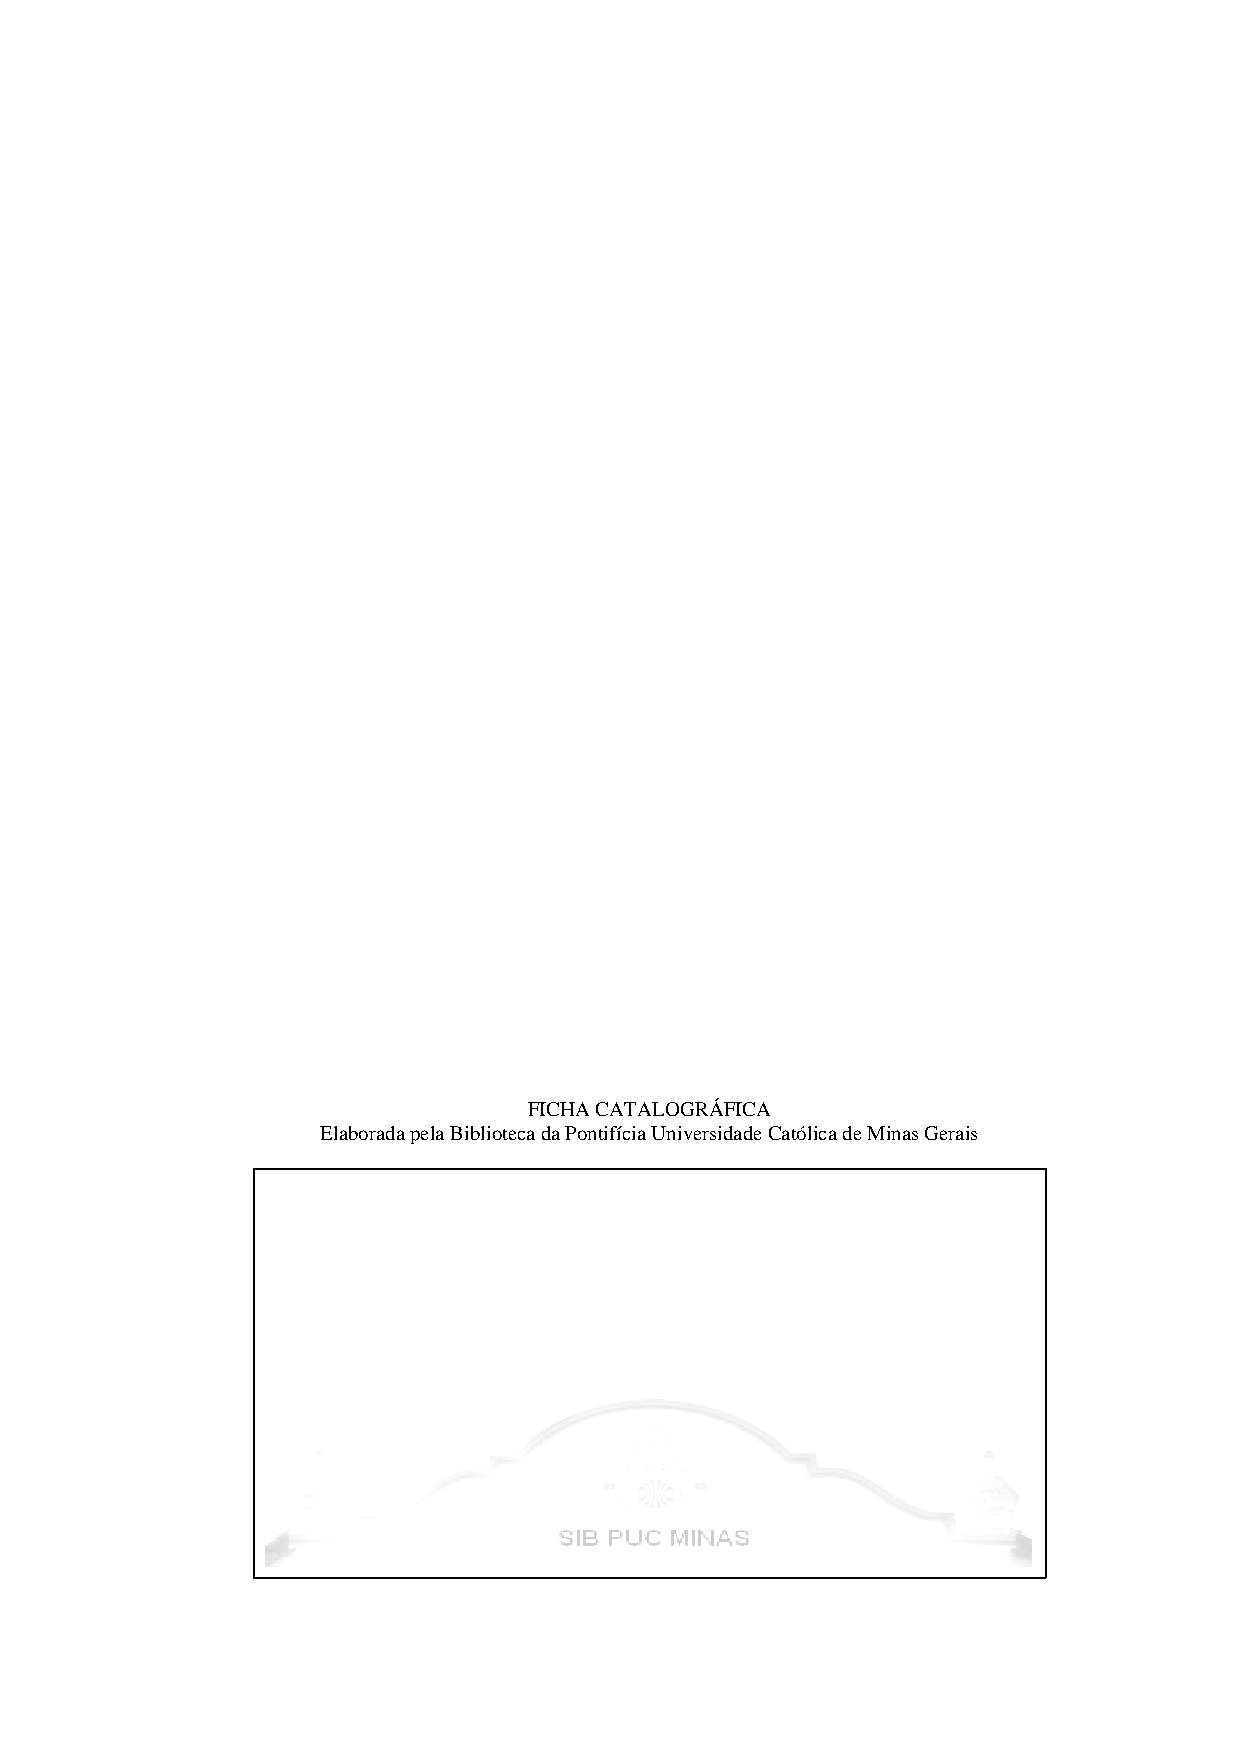
\includegraphics{pre-texto/ficha-catalografica} 
%	\newpage
%\end{figure}

% Para forçar que elementos pré-textuais (da capa até o sumário) sejam impressos no anverso da folha
\setboolean{@twoside}{false}

% Folha de aprovação
% Termo de Aprovação

% Texto da aprovação
\textoaprovacao{Monografia apresentada ao curso de Engenharia de Computação da Pontifícia Universidade Católica de Minas Gerais, como requisito parcial para obtenção do título de Bacharel em Engenharia de Computação.}

% Primeira assinatura
\primeiroassina{Prof. Dr. Orientador -- PUC Minas}

% Segunda assinatura
\segundoassina{Prof.$^{a}$ Dr.$^{a}$ Membro interno -- Instituicao}

% Terceira assinatura
\terceiroassina{Prof. Dr. Membro externo -- Instituicao}

% Quarta assinatura
%\quartoassina{}

% Data da defesa
\localdia{Belo Horizonte, data da defesa.}

% Gera o termo de aprovação
\termodeaprovacao	

% Dedicatória
% Dedicatória
\newpage

% Espaçamento do topo da página até o texto da dedicatória
\vspace*{22cm}

% Espaçamento na esqueda
\hspace{6cm}\begin{minipage}{.63\textwidth}
            \textit{Dedico este trabalho ao meu pai Jorge Durvalino, minha mãe Maria Aparecida e aos meus irmãos por me apoiarem em todos esses anos de estudos.}
            \end{minipage}

% Agradecimentos
% Agradecimentos
%\chapter*{Agradecimentos}
\begin{center}
	\normalsize
	\textbf{AGRADECIMENTOS}
\end{center}

  Texto de agradecimentos (opcional).

% Epígrafe
%% Epígrafe
\newpage

% Espaçamento entre topo da página e texto da epígrafe
\vspace*{10cm}
% Espaçamento na esqueda
\hspace{4cm}\begin{minipage}{.51\textwidth}

% Texto da epígrafe
\textit{``E fazendo que se aprende a fazer aquilo que se deve aprender a fazer.'' }

%Nome do autor
\begin{flushright}\itshape Aristoteles \upshape\end{flushright}

\end{minipage}

% Resumo
% Resumo
\begin{resumo}
% Diminuir espaçamento entre título e texto
\vspace{-1cm}

% Texto do resumo: sem paragrafo, justificado, com espaçamento 1,5 cm
\onehalfspacing

\noindent 
No mercado competitivo em que todos atuamos como profissionais, há uma constante necessidade de tomadas de decisões que podem ser cruciais para o negócio ou empresa, isso faz com que a informação seja cada vez mais importante independente do segmento de negócio. Atualmente o volume de dados cresce de maneira exponencial, sendo assim, se torna imprescindível escolher um sistema de banco de dados que seja capaz de oferecer segurança e também performance na busca das informações.

% Espaçamento para as palavras-chave
\vspace*{.75cm}

% Palavras-chave: sem parágrafo, alinhado à esquerda
\noindent Palavras-chave: Banco de dados, Desempenho, SAP, ERP, SAP HANA, \textit{Software}.\\
% Segunda linha de palavras-chave, com espaçamento.
%\indent\hspace{2cm}Palavra.

\end{resumo}

% Abstract
% Abstract
\begin{abstract}
% Diminuir espaçamento entre título e texto
\vspace{-1cm}
% Texto do resumo, em inglês: sem paragrafo, justificado, com espaçamento 1,5 cm
\onehalfspacing
\noindent
In the competitive market in which we all act as professionals, 
there is a constant need for decision making that can be crucial to the business or company, 
this makes information more and more important, independent of the business segment. Currently the volume of data grows exponentially, this is why it is imperative to choose a database system that is capable of providing security and performance in the search for information.

% Espaçamento para as palavras-chave
\vspace*{.75cm}

% Palavras-chave: sem parágrafo, alinhado à esquerda
\noindent Keywords: 
Database, Software, SAP, ERP, SAP HANA, Software. \\
% Segunda linha de palavras-chave, com espaçamento.
%\indent\hspace{1.4cm} Keyword.

\end{abstract}

\makeatletter
\renewcommand\numberline[1]{
	\leftskip 0em
	\rightskip 1.6em
	\parfillskip -\rightskip
	\parindent 0em
	\@tempdima 2.0em
	\vspace{0em} \advance\leftskip \@tempdima \null\nobreak\hskip -\leftskip
	FIGURA \normalfont #1 -- }
\makeatother

% Lista de figuras
\listoffigures

\makeatletter
\renewcommand\numberline[1]{
	\leftskip 0em
	\rightskip 1.6em
	\parfillskip -\rightskip
	\parindent 0em
	\@tempdima 2.0em
	\vspace{0em} \advance\leftskip \@tempdima \null\nobreak\hskip -\leftskip
	TABELA \normalfont #1 -- }
\makeatother

% Lista de tabelas
\listoftables

\makeatletter
\renewcommand\numberline[1]{
	\leftskip 0em
	\rightskip 1.6em
	\parfillskip -\rightskip
	\parindent 0em
	\@tempdima 2.0em
	\vspace{0.5em} \advance\leftskip \@tempdima \null\nobreak\hskip -\leftskip
	GRÁFICO \normalfont #1 -- }
\makeatother

% Lista de graficos
\listof{grafico}{Lista de Graficos}

% Lista de siglas
% Lista de Abreviaturas e Siglas
%\chapter*{Lista de Abreviaturas e Siglas}
\chapter*{Lista de Abreviaturas e Siglas}

% Mantenha sempre em ordem alfabética.
\begin{acronym} 
\acro{ECC} {\textit{ERP Central Component}}
\acro{ERP} {\textit{Enterprise Resource Planning}}
\acro{SGBD} {Sistema de Gerência de Banco de Dados}
\acro{SQL} {\textit{Structured Query Language}}
\acro{TI} {Tecnologia da Informação}
\acro{BD} {banco de dados}
\acro{NoSQL}{Not Only SQL}
\acro{MVCC} {\textit{Controle de Concorrência Multiversão}}
\acro{BT} {\textit{Block Tri-diagonal}}
\acro{CG} {\textit{Conjugate Gradient}}
\acro{CSS} {\textit{Chirp Spread Spectrum}}
\acro{DCC-MAC} {\textit{Dynamic Channel Coding} MAC}
\acro{DSSS} {\textit{Direct-sequence spread spectrum}}
\acro{EP} {\textit{Embarrassingly Parallel}}
\acro{FIFO} {\textit{First In, First Out}}
\acro{FT} {\textit{Fast Fourier Transform}}
\acro{IEEE} {\textit{Institute of Electrical and Electronics Engineers}}
\acro{IR-UWB} {\textit{Impulse Radio} UWB}
\acro{IS} {\textit{Integer Sort}}
\acro{LU} {\textit{Lower-Upper Gauss-Seidel}}
\acro{MAC} {\textit{Medium Access Control}}
\acro{MB-OFDM} {\textit{Multi-Band Orthogonal Frequency Division Multiplexing}}
\acro{MG} {\textit{Multi-Grid}}
\acro{MPE} {MPI \textit{Parallel Environment}}
\acro{MPI} {Interface de passagem de mensagem, do inglês \textit{Message Passing Interface}}
\acro{NAS} {NASA \textit{Advanced Supercomputing}}
\acro{NOAH} {\textit{No Ad-Hoc Routing Agent}} 
\acro{NS-2} {\textit{Network Simulator} 2}
\acro{NoCs} {Redes-em-Chip, do inglês \textit{Networks-on-Chip}}
\acro{NPB} {NAS \textit{Parallel Benchmark}}
\acro{OpenMP} {Multi-processamento aberto, do inglês \textit{Open Multi-Processing}}
\acro{PHY} {\textit{Physical Layer}}
\acro{PPM} {\textit{Pulse-Position Modulation}}
\acro{SP} {\textit{Scalar Penta-diagonal}}
\acro{TH} {\textit{Time Hopping}}
\acro{THS} {\textit{Time Hopping Sequence}}
\acro{UDP}{\textit{User Datagram Protocol}}
\acro{UWB} {\textit{Ultra Wide Band}}
\acro{WiNoCs} {Redes-em-Chip Sem Fio, do inglês \textit{Wireless Networks-on-Chip}}
\acro{WLAN} {Rede Local Sem Fio, do inglês \textit{Wireless Local Area Network}}
\acro{WPAN} {Rede de Área Pessoal Sem Fio, do inglês \textit{Wireless Personal Area Network}}
\end{acronym}

\makeatletter
\renewcommand\numberline[1]{#1\hspace{0.8em}}
\makeatother

% Altera para espaçamento simples a partir daqui
\singlespacing

% Sumáriox'
\tableofcontents

% Altera para espaçamento 1,5 a partir daqui
\onehalfspacing

%% TEXTUAIS 
% Para forçar que elementos textuais e pós-textuais sejam impressos no anverso e verso das folhas
%\setboolean{@twoside}{true}
% Altere o número da página para o correto. Conte todas as páginas frente e verso, menos a capa, nclusive a ficha catalográfica até a página do primeiro capítulo.
\setcounter{page}{5}

% Capítulos
% Para forçar que o capítulo de introdução comece no anverso
%\setboolean{@openright}{true}
% Nome do capítulo
\chapter{Introdução}
% Label para referenciar
\label{cap1}

% Diminuir espaçamento entre título e texto
\vspace{-1.9cm}

% Texto do capítulo
Atualmente, as empresas estão cada vez mais dependentes de tecnologias informatizadas que são responsáveis pela coleta, processamento, armazenagem, análise e distribuição de informações e dados importantes em um determinado contexto dentro do ramo de negócio. Em geral, as grandes companhias estão buscando adotar modelos de gerência para aperfeiçoar a utilização dos recursos da informação para alinha-los ao foco do negócio. \cite{WEILL}

A quantidade de informação que está disponível para a humanidade é enorme e à medida que o conhecimento humano se expande, maior é a quantidade dessa informação que precisa ser armazenada e analisada. Além da quantidade, o fluxo e a variedade dessas informações constantemente desafiam a indústria pois a quantidade de dados manipulados aumenta exponencialmente. Assim, um sistema de banco de dados eficiente se torna indispensável para qualquer tipo de negócio, pode-se classificar como sistema de banco de dados qualquer sistema, baseado em computador, que reúna, organize e mantenha informações e registros ordenados sobre um determinado assunto que seja considerado significativo à organização servida por esse sistema. \cite{datebd}


%pode-se classificar como banco de dados qualquer sistema que reúna e organize informações e registros ordenados sobre determinado assunto. Uma lista telefônica, o catálogo de livros de uma biblioteca, ou qualquer base de dados onde seja possível localizar ou gerenciar informações armazenadas são exemplos de bancos de dados.

%Basicamente nada mais é do que um sistema de armazenamento de dados baseado em computador; isto é, um sistema cujo objetivo global é registrar e manter informação. Esta informação pode ser qualquer uma considerada significativa à organização servida pelo sistema.%

Os bancos de dados e sua tecnologia tem um impacto importante sobre o uso crescente dos computadores. É correto afirmar que os bancos de dados desempenham um papel crítico em quase todas as áreas em que os computadores são usados, por exemplo: negócios, comércio eletrônico, engenharia, medicina, genética, direito, educação e biblioteconomia. \cite{navathesistemas}

No contexto corporativo, são os bancos de dados que fornecem armazenamento e gerenciamento de forma efetiva dos dados de clientes, fornecedores, produtos, pequisas, currículos, portifólios e etc. Exatamente por conta disso, a área de banco de dados, incentivada pela demanda do mercado, está em constante desenvolvimento e crescimento no mercado de \ac{TI}.

As grandes corporações e empresas sabem da importancia de possuir, interpretar e processar os dados de suas vendas, compras, finanças e por esse motivo já possuem algum sistema de gestão empresarial conhecidos como \ac{ERP}. Um sistema ERP busca a  integração  entre  as  diversas  áreas  operacionais
e gerenciais de uma empresa. Este sistema atua como espinha dorsal que se estende aos sistemas dos clientes, fornecedores e parceiros comerciais, formando uma cadeia de valor integrada ao processo de negócio. Com todas essas informações para armazenar e processar os sistemas ERPs participaram diretamente do desenvolvimento e crescimento da área de banco de dados. 

A maior parte das aplicações de banco de dados armazenam os dados nos discos rígidos, devido ao baixo custo por bit e sua natureza não volátil. Mas, a latência do acesso aos dados em disco é limitada por suas características mecânicas o que torna o acesso aos dados relativamente mais lento. 

Com o desenvolvimento tecnológio os sistemas de banco de dados baseado em disco não conseguem acompanhar os requesitos de desenpenho das aplicações modernas. E, deste mesmo modo, as memórias RAM impulsionam a curva tecnológica aumentando sua capacidade e diminuindo o custo por bit a cada geração. \cite{ravinair}
%(CITAR https://ieeexplore.ieee.org/document/7151782/references#references)

Para suprir essa demanda surgiram os banco de dados baseados em memória principal, onde os dados são alocados na memória principal do computador e não mais em discos rígidos. Dessa forma, quando os dados precisam ser analidados, já estão disponíveis instantaneamente, acelerando a velocidade de processamento.


%Um dos maiores sistemas ERP do mundo é o SAP \ac{ECC}. O SAP ECC, desenvolvido pela empresa alemã \textbf{SAP SE}, fornece módulos que abrangem uma ampla gama de processos dentro de uma empresa, incluindo finanças, logística, recursos humanos, planejamento de produtos e atendimento ao cliente, conectados em um único sistema personalizável executado em um banco de dados de escolha do usuário.  

%Contudo, no cenário corporativo o SAP ECC vem sendo substituido pelo SAP S/4 HANA, um pacote ERP projetado especificamente para computação \textit{in-memory} onde os dados são alocados na memória central do computador e não mais em discos rígidos. Desta forma, quando os dados precisam ser analisados, já estão disponíveis instantaneamente, acelerando a velocidade de processamento.

\section{Objetivos}
\label{secao1}

O objetivo deste trabalho é realizar uma pesquisa sobre os banco de dados baseados em disco e banco de dados baseados em memória principal. Realizar um estudo sobre banco de dados, compreender a estrutura de armazenamento dessas duas tecnologia, realizar comparações de desempenho de leitura e escrita, também serão realizados testes de inserção, seleção, atualização e remoção dos dados, portanto o trabalho tem como meta oferecer mais um mecanismo de comparações entres os dois modelos de \ac{BD}.  

%O objetivo deste trabalho é realizar uma pesquisa sobre banco de dados relacionais utilizados no SAP ECC e bancos de dados \textit{in-memory} utilizados no sap S/4 HANA, realizar comparações de desempenho de leitura e escrita, também serão realizados testes de inserção, seleção, atualização e remoção dos dados, portanto o trabalho tem como meta oferecer mais um mecanismo de comparações entres os dois modelos de \ac{BD}.  

%é apresentar uma comparação do desempenho dos bancos de dados utiliazados nos sistemas de gestão empresarial SAP ECC e SAP S/4 HANA, apresentando os principais conceitos e caracteristicas de cada banco de dados e realizar comparações quanto ao tempo de inserção, seleção, atualização e remoção de dados.%

Dentre os objetivos específicos, tem-se:

	\begin{compactitem}
      \item[a)] Apresentar as principais diferenças entre os dois bancos de dados;
      \item[b)] Apresentar um estudo de caso dos dois BDs
      \item[c)] Criar e popular tabelas para realização dos testes;
      \item[d)] Capturar o tempo de execução de cada uma das interação com os bancos de dados;
      \item[e)] Analisar os resultados;
    \end{compactitem}

\section{Justificativa}
\label{secao2}

As grandes empresas de todo o mundo executam milhares de transações por dia, realizando compras e vendas, recenbendo novos produtos, vendendo outro produtos e serviços, realizando pagamentos, gerenciando contas de pessoas e etc. Como todas essas informações já estão automatizadas e armazenadas em bancos de dados, é muito importante saber qual irá gerar uma maior economia de tempo, diminiução dos custos e maior produtividade, gerando assim mais lucro. 

Além disso, compreender o funcionamento de cada banco de dados pode auxiliar também os desenvolvedores, por terem um maior embasamento teórico no momento de escolher o \ac{SGBD} que irão utilizar no desenvolvimento de suas aplicações. 



\section{Organização do trabalho}
% - Apresentar os banco de dados - Falar sobre tecnologias opensource

O trabalho consistem em realizar um estudo sobre banco de dados comparando as abordagens utilizadas nos banco de dados baseados em disco e nos banco de dados baseados em memória principal. Para isso buscou-se uma revisão bibliográfica para entendiento dos principais conceitos que precisan ser entendidos para as análises dos resultados. 

O banco de dados baseado com o armazenamento em disco utilizado neste trabalho foi o PostgreSQL, um poderoso sistema de banco de dados relacional de código-fonte aberto que utiliza a linhaguem SQL. O PostgreSQL possui mais de 30 anos de desenvolvimento ativo e por isso é bastante confiável para este estudo. 

Por sua vez, o Redis foi o banco de dados com armazenamento de dados baseado em memória principal utilizado neste estudo. O Redis também foi escolhido por ser \textit{open source}.

A metodologia de pesquisa trata-se de uma forma descritiva de busca de dados e indicações para análise. Os resultados são avaliados de maneira a conferir os dados encontrados com análises dos dados coletados durante o desenvolvimento do trabalho. 

%O trabalho consiste em realizar um estudo sobre o banco de dados utilizado no SAP ECC e o banco de dados utilizado no SAP S/4 HANA e comparar o desempenho de dois bancos de dados. Para isso buscou-se uma revisão bibliográfica para entendimento dos principais conceitos que precisam ser entendidos para as análises de resultados. A metodologia de pesquisa trata-se de uma forma descritiva de busca de dados e indicações para análise. Os resultados são avaliados de maneira a conferir os dados encontrados com análises dos dados coletados durante o desenvolvimento do trabalho. 

\subsection{Fundamentação teórica}

A fundamentação teórica basicamente se divide em três partes. A primeira analisa de maneira clara e objetiva os conceitos relacionados a banco de dados que são premissas para o entendimento deste trabalho. 

A segunda parte aborda abora da história dos dois banco de dados escolhidos para realização deste trabalho (\textit{PostgreSQL e Redis}), a fim de contexualizar sobre a finalidade de uso desses banco de dados. 

A terceira parte faz referência aos estudos já realizados nessa área da tecnologia, afim de entender a metodologia utilizada por outros autores com o objetivo de embasar a metodologia científica empregada nesse estudo. 

\subsection{Metodologia}
O  capitulo  de  metodologia  se  concentra  em  esclarecer  as  técnicas  de  pesquisa adotadas  para  obtenção  dos  resultados.  São expostos nessa parte do trabalho como foi feito a população das tabelas, coleta dos dados e análise dos resultados. Assim o capítulo se divide em: 

\begin{compactitem}
	\item Criar as tabelas.
    \item Popular as tabelas.
    \item Coleta dos dados.
    \item Análise e conferência dos dados coletados.
\end{compactitem}

\subsection{Testes e Resultados}
Esse capítulo trata de expor os resultados encontrados com a pesquisa descrita na metodologia. Dividindo-se em duas partes: análise dos tempos de execução coletados em cada um dos bancos de dados separadamente e comparação dos dados coletados de um banco de dados com o outro.

Na primeira parte serão expostos em tabelas o tempo que cada sentença SQL demorou para ser executado e realização de análise sobre estes dados. Já na segunda os dados de cada banco de dados serão confrontados para análise de desempenho.

\subsection{Conclusão}
A conclusão aponta as diferenças no desempenho dos banco de dados e também  Sugestões  para  outros trabalhos são propostas a partir da temática desenvolvida. 





%Atualmente, há uma grande busca por desenvolver aplicações e sistemas que tornem a vida do usuário cada vez mais simples, tomando sempre menos tempo do dia do cliente, usuário ou paciente, melhorarando assim a qualidade de vida. 

%Além disso, é possível pensar em diversas razões para desenvolver um projeto deste tipo, pois criando aplicações inteligentes que sejam capazes de realizar diagnósticos precisos é possível melhorar as condições de trabalho para os médicos ou fisioterapeutas, que terão maior confiança em indicar um tratamento para seus pacientes. 

%Quando se fala em medicina e fisioterapia sempre se tem em mente equipamentos modernos e caros, o que dificulta o acesso de pessoas de baixa renda a estes exames. Portanto, há uma grande necessidade em aumentar o número de \textit{softwares} e aplicações que sejam simples e eficazes no diagnóstico do paciente. Possibilitando, assim, o acesso de um maior número de pessoas a estes exames.


%A seguir serão apresentados alguns comandos do LaTex usados comumente para formatar textos de dissertação baseados
%  na normalização da PUC (2011).

%   Para as citações a norma estabelece duas formas de apresentação. A primeira delas é empregada quando a
%   citação aparece no final de um parágrafo. Neste caso, o comando cite é usado para formatar a citação em caixa alta,
%  como é mostrado no exemplo a seguir. \cite{Duato:2002}.

%   Outra forma de apresentação da citação é a que ocorre no decorrer do texto, essa situação é exemplificada na próxima frase.
%   Conforme \citeonline{Bjerregaard:2006}, o estudo mencionado revela progressos no desempenho dos processadores. 
%   Para a formatação da citação em caixa baixa deve ser usado o comando citeonline.

%   Nas citações que aparecem mais de uma referência as mesmas devem ser separadas por vírgulas, como
%   neste exemplo. \cite{Keyes:2008, Zhao:2008, Ganguly:2011}. Se houver necessidade de especificar a página ou que foi
%   realizada uma tradução do texto deve ser feito da seguinte maneira. \cite[p.~2, tradução nossa]{Sasaki:2009}.
 %  A citação direta deve ser feita de forma semelhante. ``[...] A carga de trabalho de um sistema pode 
%   ser definida como o conjunto de todas as informações de entrada.''~\cite[p. 160]{Menasce:2002}.

%   O arquivo dissertacao.bib mostra exemplos de representação para vários tipos de referências (artigos de conferências, 
%   periódicos, relatórios, livros, dentre outros). Cada um desses tipos requer uma forma diferente de representação para 
%   que a referência seja formatada conforme as exigências da normalização.


% \subsection{Primeira subseção}
  
%   As enumerações devem ser geradas usando o pacote \textit{compactitem}. Cada item deve terminar com um ponto final.
 %  Abaixo um exemplo de enumeração é apresentado:
% 
   %  \begin{compactitem}
%       \item[a)] Coletar e analisar.
%       \item[b)] Configurar e simular.
%       \item[c)] Definir a metodologia.
%       \item[d)] Avaliar o desempenho.
%       \item[e)] Analisar e avaliar características.
%     \end{compactitem}
%
%\section{Segunda seção}

%  Para referenciar um capítulo, seção ou subseção basta definir um label para o mesmo e usar o comando ref para referênciá-lo
%  no texto. Exemplo: Como pode ser visto no Capítulo \ref{cap1} ou na Seção \ref%{secao1}.
% Os demais capítulos não precisam começar no anverso
\setboolean{@openright}{false}
% Nome do capítulo
\chapter{Fundamentação Teórica}
% Label para referenciar
\label{cap2}

% Diminuir espaçamento entre título e texto
\vspace{-1.9cm}

% Texto do capítulo
Neste capítulo, serão abordados os conceitos importantes e necessários para o entendimento do propósito do trabalho, tais como sistema de gerenciamento de bando de dados SGBD, tipos de banco de dados e as diferênças entre eles.


\section{Banco de dados}
Um banco de dados basicamente é um sistema de armazenamento de dados baseado em computador; isto é, um sistema cujo objetivo global é registrar e manter informações. Estas informações pode ser qualquer uma considerada significativa para à empresa ou organização \cite{datebd}. Uma coleção de informações que se relacionam de modo que criem algum sentido, ou seja, é uma estrutura bem organizada de dados que permite a extração de informações. 

Banco de dados são amplamente utilizados, como exemplo de aplicações podemos citar: 

\begin{itemize}
    \item Informações de empresas
        \begin{itemize}
            \item Vendas: Informações sobre clientes, produtos e pedidos compras
            \item Contabilidade: Pagamentos, recebimentos, saldos de conta, ativos e outras informações contábeis.
            \item Recursos humanos: Informações sobre funcionários, salários e impostos sobre folha de pagamento.
            \item Fabricas: Gerenciamento da cadeia de suprimentos e para rastrear a produção de itens nas fábricas, estoques de itens em armazéns e lojas e pedidos de itens.
        \end{itemize}
    
    \item Bancos e sistemas financeiros
        \begin{itemize}
            \item Bancos: Informações sobre clientes, contas, empréstimos e transações bancárias.
            \item Transações com cartão de crédito: Informações de compras em cartões de crédito e geração de extratos mensais.
        \end{itemize}
    
    \item Universidades: Para informações sobre os alunos, registros de cursos e notas (além de informações corporativas padrão, como recursos humanos e contabilidade).
    
    \item Companhias aéreas: Informações sobre reservas e informações de agendamento. As companhias aéreas estavam entre as primeiras a usar bancos de dados de maneira geograficamente distribuída.   
    
    \item Telecomunicação: Para manter registros de chamadas feitas, gerar contas mensais, manter saldos em contas pré-pagas e armazenar informações sobre as redes de comunicação.

\end{itemize}

- A referencia do livre Data base System Concepts 7 edição está nesse link
%https://www.campusbookrentals.com/textbook/database-system-concepts-7th-edition-silberschatz/9789332901384
- Contextualizar e finalizar seção

%Podemos exemplificar situações clássicas como uma lista telefônica, um catálogo de livros de uma biblioteca ou um sistema de controle de RH de uma empresa.

\section{Sistema de Gerência de Banco de Dados }

Segundo \citeonline{carlos} um Sistema de Gerência de Banco de Dados (\ac{SGBD}) é um software que incorpora as funções de definição, recuperação e alteração de dados em um banco de dados. Seu principal objetivo é retirar da aplicação cliente a responsabilidade de gerenciar o acesso, a manipulação e a organização dos dados. O SGBD disponibiliza uma interface para que seus clientes possam incluir, alterar ou consultar dados previamente armazenados. 

Portanto, \ac{SGBD} é um software projetado para auxiliar a manutenção e utilização de vastos conjuntos de dados. \cite{ramakrishnan2008sistemas} O uso de um SGBD possui, entre outras, as seguintes vantagens: 

\begin{compactitem}
    \item \textbf{Independência de dados:} As aplicações não devem, idealmente, ser expostos aos detalhes de representação e armazenamento de dados. O SGBD provê uma visão abstrata dos dados que oculta tais detalhes. 
    
    \item \textbf{Acesso eficiente aos dados:} Um SGBD utiliza uma variedade de técnicas sofisticadas para armazenar e recuperar dados eficientemente. Este recurso é especialmente importante se os dados são armazenados em dispositivos de armazenamento externos. 
    
    \item \textbf{Integridade e segurança dos dados:} Se os dados são sempre acessados através do SGBD, ele pode forçar restrições de integridade. Por exemplo, antes de inserir informações sobre o salário de um funcionário, o SGBD pode verificar se o orçamento do departamento não está se excedendo. Além disso, ele pode formar controles de acesso que governam quais dados estão visíveis a diferentes classes de usuários. 
    
    \item \textbf{Administração de dados:} Quando diversos usuários compartilham dados, centralizar a administração dos dados pode oferecer melhorias significativas. Profissionais experientes que compreendem a natureza dos dados sendo gerenciados, e como os diferentes grupos de usuários os utilizam, podem ser responsáveis por organizar a representação dos dados para minimizar a redundância e para realizar as sintonizações finais do armazenamento dos dados para garantir uma eficiente recuperação. 
    
    \item \textbf{Acesso concorrente e recuperação de falha:} Um SGBD planeja o acesso concorrente aos dados de maneira tal que os usuários podem achar que os dados estão sendo acessados por apenas um único usuário de cada vez. Além disso, o SGBD protege os usuários dos efeitos de falhas de sistema. 
    
    \item \textbf{Tempo reduzido de desenvolvimento de aplicações:} Obviamente, o SGBD suporta funções importantes que são comuns a vários aplicativos que acessam os dados no SGBD. Isso, em conjunto com uma interface de alto nível, facilita o desenvolvimento rápido de aplicativos. Os aplicativos de SGBD tendem a ser mais robustos do que os palicativos similires independentes porque muitas tarefas importantes são tratadas pelo SGBD e não precisam ser depuradas e testadas no aplicativo. 
\end{compactitem}

\section{Banco de dados relacional}

De acordo com \citeonline{navathesistemas} O modelo de dados relacional foi introduzido inicialmente por Edgar Frank Codd, da IBM Research, em 1970, em um artigo \cite{codd}, que atraiu atenção imediata devido a sua simplicidade e base matemática.

O Modelo Relacional é um modelo matemático derivado da Teoria dos Conjuntos que propõe que as estruturas de dados devem ser encaradas como conjuntos. Segundo essa teoria, entendemos por conjunto o agrupamento de elementos que possuem características semelhantes, coleção de objetos. 

O modelo relacional representa o banco de dados como uma coleção de relações. Informalmente, cada relação é semelhante a uma tabela de valores. Em uma tabela de valores cada linha na tabela representa uma coleção de valores de dados relacionados. Uma linha representa um fato que normalmente corresponde a uma entidade ou relacionamento no mundo real. Os nomes da tabela e da coluna são usados para ajudar a interpretar o significado dos valores em cada linha. 

Na Figura \ref{fig:1}. a tabela é chamada de ALUNO porque cada linha representa fatos sobre uma entidade particular de aluno. Os nomes de coluna (Cpf, Endereco, Media, etc.) especificam como interpretar os valores de dados em cada linha, com base na coluna em que cada valor se encontra. Todos os valores em uma coluna são do mesmo tipo de dados. Na terminologia formal do modelo relacional, uma linha é chamada de tupla, um cabeçalho da coluna é chamado de atributo e a tabela é chamada de relação.

\begin{figure}[H]
  % Alterar espaçamentos antes e depois do caption
  \setlength{\abovecaptionskip}{0pt}
  \setlength{\belowcaptionskip}{0pt}
  % Caption
  \caption[Atributos e tuplas de uma relação ALUNO]{Atributos e tuplas de uma relação ALUNO}
  \centering
  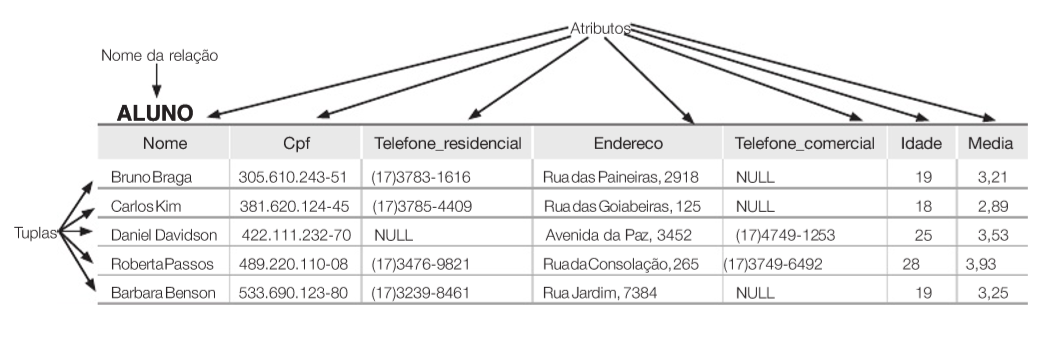
\includegraphics[width=.95\textwidth]{imagem/RelationalTable.png}
  % Caption centralizada
  \captionsetup{justification=centering}
  \captionfont{\small{\textbf{\\Fonte: \cite{navathesistemas} }}}	
  \label{fig:1}
\end{figure}





%Um banco de dados relacional é uma coleção de dados com relacionamentos predefinidos entre si. Esses itens são organizados como um conjunto de tabelas com colunas e linhas. As tabelas são usadas para reter informações sobre os objetos a serem representados no banco de dados. Cada coluna da tabela retém um determinado tipo de dado e um campo armazena o valor em si de um atributo. As linhas na tabela representam uma coleção de valores relacionados de um objeto ou uma entidade. Cada linha em uma tabela pode ser marcada com um único identificador chamado de chave principal. Já as linhas entre as várias tabelas podem ser associadas usando chaves estrangeiras. 



%Os bancos de dados relacionais são fundamentados no paradigma da orientação a conjuntos, uma vez que sua base é contruída em cima da teoria de conjuntos. Esses bancos de dados armazenam dados em estruturas chamadas tabelas, compostas por colunas e linhas. Sua linguágem é a \ac{SQL}. \cite{impacta}

%O modelo de banco de dados relacional é o mais utilizado atualmente no mercado e um dos principais motivos para isso é a preocupação com a consistência dos dados, no qual é garantida pelo princípio conhecido como ACID, Atomicidade, Consistência, Isolamento e Durabilidade. Esse princípio pode ser definido como:

%\begin{compactitem}
%	\item \textbf{Atomicidade}: Trata a transação como parte indivisível, A transação deve ter todos os registros alterados em caso de sucesso ou, em caso de falha, nenhum registro deve ser alterado, garantindo que nenhuma alteração fique incompleta. 
    
%    \item \textbf{Consistência}: A execução de uma transação deve levar ao banco de dados de um estado consistente a outro também consistente. Uma transação é consistente se não violar a integridade do banco de dados. Se a transação tiver êxito ou falhar, ela deve deixar o banco de dados em um estado consistente.Se uma transação falhar, ela precisa desfazer todas as alterações temporárias e deixar o banco de dados no estado em que ele estava antes que a transação iniciou.
    
%    \item \textbf{Isolamento}: Uma transação em andamento mas ainda não validada deve permanecer isolada de qualquer outra operação, ou seja, garantimos que a transação não será interferida por nenhuma outra transação concorrente
    
%    \item \textbf{Durabilidade} Os efeitos de uma transação em caso de sucesso devem persistir no banco de dados mesmo em casos de quedas de energia, travamentos ou erros. Garantindo que os dados estarão disponíveis em definitivo.     
%\end{compactitem}

\section{Banco de Dados não relacional}
Um banco de dados não relacional é um banco de dados que não utiliza o esquema de tabela de linhas e colunas encontrado no modelo relacional. Em vez disso, os bancos de dados não relacionais usam um modelo de armazenamento otimizado para os requisitos específicos do tipo de dados que está sendo armazenado.

Os bancos de dados não relacionais também são conhecidos como \ac{NoSQL}. O Termo NoSQL, foi utilizado pela primeira no final dos anos 90, por Carlo Strozzi, como nome de seu SGBD, baseado no Modelo Relacional, sem interface SQL. Sendo uma solução alternativa para os bancos de dados relacionais. Os banco de dados \ac{NoSQL} possuem uma alta escalabilidade, disponibilidade,  desempenho e menor tempo de resposta a consultas. \cite{nosqlpramod}


Os bancos de dados não relacionais foram construídos baseados nas seguintes classificações: 
\begin{compactitem}
	\item \textbf{Bancos de dados orientados à documentos}: No modelo orientado a documentos tem-se um esquema que representa o documento e em cada documento tem-se um conjunto de campos chave que o identifica. Esse documento não depende de um esquema rígido, ou seja, não exige uma estrutura fixa como ocorre nos bancos relacionais. Assim, é possível que ocorra uma atualização na estrutura do documento, com a adição de novos campos, por exemplo, sem causar problemas ao banco de dados. Na Figura \ref{fig:2} o documento é representado por uma estrutura JSON (JavaScript Object Notation).  
	
\begin{figure}[H]
  % Alterar espaçamentos antes e depois do caption
  \setlength{\abovecaptionskip}{0pt}
  \setlength{\belowcaptionskip}{0pt}
  % Caption
  \caption[Banco de dados de Documentos]{Armazenamento de dados de Documentos}
  \centering
  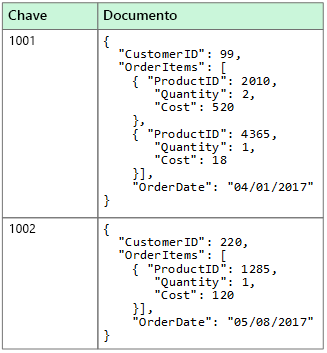
\includegraphics[width=.65\textwidth]{imagem/NoSQL_Document.png}
  % Caption centralizada
  \captionsetup{justification=centering}
  \captionfont{\small{\textbf{\\Fonte: \cite{microsoft} }}}	
  \label{fig:2}
\end{figure}
    
    \item \textbf{Bancos de dados orientados a colunas}: Esse modelo de banco de dados é parecido, conceitualmente com os bancos de dados relacionais, entretanto, ao invés de cada registro da tabela ficar armazenado em uma linha, o registro passa a ser armazenado em colunas separadas. Essa forma de armazenamento possui a vantagem de que cada coluna irá conter o mesmo tipo de dado, conforme demonstrado na Figura \ref{fig:3}. 
    
\begin{figure}[H]
  % Alterar espaçamentos antes e depois do caption
  \setlength{\abovecaptionskip}{0pt}
  \setlength{\belowcaptionskip}{0pt}
  % Caption
  \caption[Banco de dados de colunas]{Armazenamentos de dados de colunas}
  \centering
  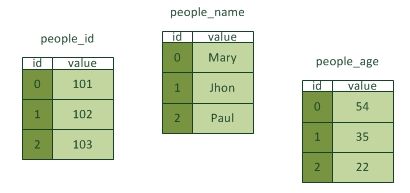
\includegraphics[width=.65\textwidth]{imagem/NoSQL_Column.png}
  % Caption centralizada
  \captionsetup{justification=centering}
  \captionfont{\small{\textbf{\\Fonte: \cite{isaias} }}}	
  \label{fig:3}
\end{figure}
    
\item \textbf{Bancos de dados de esquema Chave/Valor}: Um banco de dados de chave-valor armazena dados como um conjunto de pares de chave-valor em que uma chave funciona como um identificador exclusivo.\cite{amazon} Portanto, esse tipo de banco de dados  armazena objetos indexados por chaves e possibilitam a busca por esses objetos a partir de suas chaves, conforme demonstrado na Figura \ref{fig:4}.

\begin{figure}[H]
  % Alterar espaçamentos antes e depois do caption
  \setlength{\abovecaptionskip}{0pt}
  \setlength{\belowcaptionskip}{0pt}
  % Caption
  \caption[Banco de dados de Chave/Valor]{Banco de dados de Chave/Valor}
  \centering
  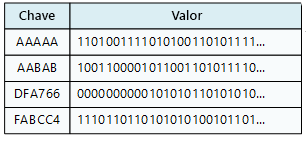
\includegraphics[width=.65\textwidth]{imagem/NoSQL_Key_Value.png}
  % Caption centralizada
  \captionsetup{justification=centering}
  \captionfont{\small{\textbf{\\Fonte: \cite{microsoft} }}}	
  \label{fig:4}
\end{figure}

\item \textbf{Bancos de dados de Graficos}: Este modelo de banco de dados armazena dois tipos de informações: nós e bordas. Os nós representam entidades e as bordas especificam as relações entre essas entidades. Ambos os nós e as bordas podem ter propriedades que fornecem informações sobre esse nó ou borda, semelhante às colunas em uma tabela. As bordas também podem ter uma direção indicando a natureza do relacionamento. A Figura \ref{fig:5} mostra um exemplo desse modelo. 

\begin{figure}[H]
  % Alterar espaçamentos antes e depois do caption
  \setlength{\abovecaptionskip}{0pt}
  \setlength{\belowcaptionskip}{0pt}
  % Caption
  \caption[Banco de dados de gráficos]{Banco de dados de gráficos}
  \centering
  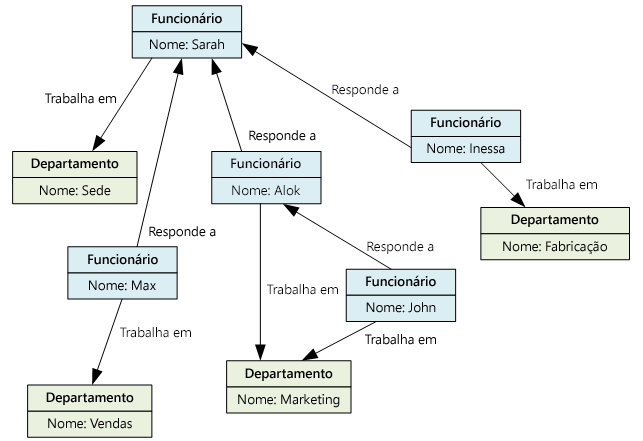
\includegraphics[width=.65\textwidth]{imagem/NoSQL_Graficos.png}
  % Caption centralizada
  \captionsetup{justification=centering}
  \captionfont{\small{\textbf{\\Fonte: \cite{microsoft} }}}	
  \label{fig:5}
\end{figure}
\end{compactitem}


\section{Banco de dados In-Memory}
Os banco de dados em memória principal armazenam os dados na memória física principal, diferentemente de um sistema de banco de dados convencional que armazena os dados no disco. Fornecendo uma maior velocidade de acesso aos dados. \cite{garcia}

Recentemente, dois fatores tornaram os bancos de dados em memória principal interessantes: os preços de memória e o paralelismo multi-core. Nos últimos 30 anos, os preços de memória baixaram 10 vezes a cada 5 anos. 

O paralelismo, juntamente com a capacidade de praticamente armazenar dados na memória, trouxe uma grande quantidade de  pesquisas e desenvolvimentos para os bancos de dados da memória principal. O resultado desse grande interesse sobre o assunto fez com que a maioria dos principais fornecedores de banco de dados desenvolvessem uma solução de banco de dados em memória, como SAP HANA, OracleTimesTen e Microsoft SQL Server Hekaton. Além disso, várias startups como o VoltDB e o MemSQL criaram um nicho no panorama do fornecedor de banco de dados.

O resultado destas pesquisas e desenvolvimentos é uma nova geração de sistemas de bancos de dados com um design bastante diferente quando comparado a um sistema relacional tradicional baseado em disco. Esses sistemas abandonam muitos dos princípios do design de livros didáticos em favor de abordagens novas, ou revisitadas, para alcançar alto desempenho em hardware moderno. \cite{Faerber}


\section{Diferenças entre banco de dados relacional e banco de dados \textit{In-memory}}


Nessa seção são avaliadas as diferenças de arquiteturas dos bancos de dados relacionais com os bancos de dados em memória principal, afim de compreender os pontos que permitem que os bancos de dados em memória principal alcancem um alto desempenho. 

\subsection{Organização e layout de dados}

Esta seção aborda os pontos básicos de organização e layout nos principais sistemas de banco de dados.

\subsubsection{Organização de dados nos banco de dados relacionais}

Quando os bancos de dados relacionais foram desenvolvidos a memória era um recuso escasso, com isso os banco de dados foram implementados sabendo que não seria possível armazenar todos os dados na memória principal. Portanto nos banco de dados relacionais os dados são armazenados no disco rígido. 

O armazenamento de dados no disco rígido implica que os dados devem ser paginados na memória conforme apropriado durante o processamento. A paginação é uma técnica utilizada para o gerenciamento de memória pelo qual o computador armazena e recupera os dados do disco rígido para usa-los na memória principal. Os blocos de dados que transitam entra a memória principal e o disco são chamados de páginas por possuírem um tamanho fixo. \cite{tanenbaum}

Os dados de paginação de/para o disco são manipulados pelo mecanismo de armazenamento do banco de dados. Além disso, as páginas são armazenadas em um conjunto de buffers compartilhados conforme a Figura 6.

\begin{figure}[H]
% Alterar espaçamentos antes e depois do caption
  \setlength{\abovecaptionskip}{0pt}
  \setlength{\belowcaptionskip}{0pt}
% Caption
  \caption[Conjunto de Buffer]{Conjunto de Buffer}
  \centering
  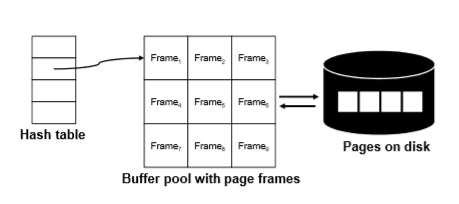
\includegraphics[width=.85\textwidth]{imagem/buffer_pool.jpg}
% Caption centralizada
  \captionsetup{justification=centering}
  \captionfont{\small{\textbf{\\Fonte: \cite{Faerber}}}}	
  \label{fig:ComponentesWiNoC}
\end{figure}

Quando o mecanismo de armazenamento recebe uma solicitação de página, ele primeiro realiza uma pesquisa na tabela de hash para determinar se a página reside no conjunto de buffers de dados. Se a página não estiver na memória, o mecanismo de armazenamento emitirá uma solicitação para trazer a página do disco para o conjunto de buffers de dados. Em seguida, ele retorna um ponteiro para o quadro da página na memória. Essa solução é solução interassante para o problema da paginação, no entanto, é facil perceber que o disco precisará ser acessado sempre que uma página não estiver no conjunto de buffers de dados afetando o desempenho dos principais sistemas de banco. 

\subsubsection{Organização de dados em sistemas de memória principal}

O principal local para registros em bancos de dados de memória principal é a RAM. Esses sistemas não são limitados pela necessidade de paginar dados de/para o disco sob demanda durante o processamento da consulta. É por essa razão que os bancos de dados modernos de memória principal evitam a estratégia baseada em página através de um conjunto de buffers de dados. Os banco de dados em memória principal não utilizam identificadores lógicos como id de página e offset, como é feito nos banco de dados trancidicionais. Em vez disso, os registros são acessados diretamente através da utilização de ponteiros. 

\subsubsection{Benefícios de desempenho ao evitar a paginação}

Evitar a estratégia do conjunto de buffer de dados para a paginação pode melhor o desempenho do banco de dados pelos seguintes motivos: 

\begin{compactitem}
    \item[(1)] Acessar os registros através do conjunto de buffer de dados leva uma sobrecarga desnecessária em um sistema  de memória principal, como pode ser visto na Figura 6, este tipo de estratégia requer duas camadas de processamento para resolver um ponteiro do registro físico, Acessando o conjunto de buffer de dados através da tabela Hash e caso seja necessário, calcular um ponteiro para o registro no disco rígido. 
    
    \item[(2)] Trava da página, o recurso que estiver acessando determinada página deverá definir uma trava de página compartilhada em caso de leitura ou um trava de página exclusiva em caso de uma atualização. A manipulação dessas travas no nível de página pode se tornar um gargalo.  

\end{compactitem}

\subsubsection{Opções de organização para sistemas modernos de memória principal}
Embora o acesso direto a registros por ponteiros seja comum entre os sistemas modernos de memória principal, eles diferem em como os registros são organizados na memória. Esse tópico resume três opções organizacionais comuns entre os banco de dados \textit{in-memory}. 

\textbf{Particionamento.} Uma das maiores diferenças entre os sistemas de banco de dados \textit{in-memory} é se eles particionam fisicamente o bando de dados ou não. H-Store e VoltDB são exemplos de sistemas particionados, enquanto Hekaton, HANA, MemSQL e Oracle TimesTen são sistemas não particionados. 
 
 
Uma partição é uma divisão de um banco de dados lógico ou seus elementos constituintes em partes independentes distintas. O particionamento de banco de dados normalmente é feito para fins de gerenciamento, desempenho ou disponibilidade, ou para balanceamento de carga. Uma aplicação popular de particionamento está em um sistema de gerenciamento de banco de dados distribuído. Cada partição pode ser distribuída em vários nós e os usuários no nó podem realizar transações locais na partição. \cite{Navathe} 
    
    
A vantagem do particionamento é que simplifica muito os problemas de simultaneidade entre threads e transações. Por exemplo, sistemas particionados, como o H-Store, executam transações em série dentro de uma partição, evitando assim protocolos de controle de simultaneidade de transações para transações de partição única
    
A vantagem de uma abordagem não particionada é que qualquer thread pode acessar e atualizar qualquer registro na base de dados.Esses sistemas evitam, assim, problemas de balanceamento de carga que podem surgir devido a partições que contém os dados mais utilizadoos, o que geralmente requer reatribuição de carga de trabalho entre os threads e possivelmente a movimentação de dados.
    
    
\textbf{Multiversão.} Uma segunda opção arquitetural importante é se os sistemas suportam multiversão de dados. Multiversão, trata-se de um controle de concorrência que utiliza a data e a hora para registrar uma cópia temporária do banco de dados no instante em que um processo é executado.  Qualquer alteração que esteja sendo feita em determinado momento por um processo, não será vista pelos demais processos operando no banco de dados, até que as alterações tenham sido confimadas. Quando um banco de dados com controle de concorrência multiversão precisar atualizar um determinado dado, ele não irá sobrescrever este dado com o novo dado, mas sim, marcar o dado antigo como obsoleto e adicionar a versão mais recente em outro lugar. Desta forma, existem várias versões armazenadas, mas apenas uma é a última. Isso permite que os processos leitores do banco dados acessem os dados que estavam lá quando eles começaram a ler, mesmo que este dado tenha sido modificado ou excluído por outro processo. \cite{Bernstein}

O \ac{MVCC} permite que os leitores nunca bloquiem os escritores e esse comportamento sem bloqueio leva a uma menor sobrecarga em comparação com os protocolos baseados em bloqueio, consequentemente uma melhora de desempenho. 


\subsection{Indexação}



%Por exemplo, os exemplos a seguir fornecem uma ideia de como esses sistemas são diferentes.

%\begin{compactitem}
    
%    \item \textbf{Organização e indexação de dados.} Uma tendência generalizada em todos os sistemas é evitar o armazenamento baseado em páginas através de um buffer pool e armazenar apenas registros na memória. Os índices geralmente armazenam apontadores diretos nos registros. Vários sistemas também implementam novos métodos de indexação que otimizam a eficiência do cache da CPU.
    
%    \item \textbf{Controle de concorrência.} A maioria dos sistemas evita o controle de simultaneidade baseado em bloqueio pessimista devido ao bloqueio e alternância de contexto. Em vez disso, alguns sistemas usam uma variante de controle de simultaneidade de várias versões, enquanto outros usam a distribuição seriada particionada para obter alto desempenho.
    
%    \item \textbf{Durabilidade e recuperação.} log e recuperação raramente são usados. Em vez disso, a maioria dos sistemas optam por uma forma de criação de log através de comando juntamente a instantâneos periódicos do banco de dados para se recuperar de uma falha ou reinicialização (Melhorar Traduçao).

%\item \textbf{Processamento e compilação de consultas.} Para evitar a sobrecarga de chamadas de função virtual, degradação da previsão de ramificação e interpretação de bytes, vários sistemas abandonam o modelo de processamento do iterador "get next". Em vez disso, as consultas são compiladas em código de máquina altamente otimizado e executadas diretamente em registros na memória 
%\end{compactitem}





CONTINUAR DAQUI











%\section{Sistema de gerenciamento de banco de dados (SGBD)}
%Um sistema de gerenciamento de banco de dados (SGBD) é uma coleção de programas que permite aos usuários criar e manter um banco de dados. O SGBD é, portanto, um sistema de software de propósito geral que facilita os processos de definição, construção, manipulação e compartilhamento de bancos de dados entre vários usuários e aplicações.\cite{navathesistemas}


\section{ERP (Enterprise Resource Planning)}
Um software ERP é um sistema de informática responsável por cuidar de todas as operações diárias de uma empresa, desde o Faturamento até o balanço contábil, de Compras a fluxo de caixa, de apuração de impostos a Administração de Pessoal, de inventário de estoque às contas a receber, do ponto dos funcionários a controle do maquinário da fábrica, portanto, todo o trabalho administrativo e operacional feito numa empresa. \cite{portalerp}

%\section{SAP}
%Empresa alemã fundada em 1972 na cidade de Walldorf, é lider de mercado no setor de desenvolvimento de softwares para gestão empresarial. A sigla SAP significa Análise de sistemas, aplicações e desenvolvimento de programas (Systemanalyse, Anwendungen und Programmentwicklung)

\section{SAP ECC}
SAP ERP Central Component (SAP ECC) é um sistema integrado de gestão empresarial (ERP). O principal produto da SAP foi projetado para ser executado em um banco de dados de terceiros, como o Oracle ou MySql.

O sistema procura contemplar a empresa como um todo, dividindo em módulos, onde cada módulo corresponde a uma área especifica, como por exemplo, o módulo SD (Sales and Distribution) que contempla a área de Vendas e Distribuição. Quando informações são alteradas em módulo do SAP um acionador atualizará as informações em outras áreas relevantes da empresa, como por exemplo o estoque. \cite{ecc}



\section{SAP HANA}

O SAP HANA é uma plataforma completa de desenvolvimento de bancos de dados e aplicativos. Ele combina um banco de dados compatível com ACID com análises de alta velocidade, serviços de aplicativos e ferramentas flexíveis de aquisição de dados. \cite{hana}

HANA significa High Performance Analytical Appliance (ferramenta analítica de alto desempenho) foi desenvolvido para aplicativos analíticos que podem ser implementados em alta velocidade. Utilizando a tecnologia in-memory o bando de dados SAP HANA se torna muito interesante para alplicações de Big Data. \cite{pelissari}

\section{SAP S/4 Hana}

SAP S/4 Hana é a abreviatura de SAP Business Suite 4 SAP HANA. O nome indica que esta é a quarta versão do SAP Business Suite, no entanto ela foi desenhada para ser executada unicamente no bando de dados SAP HANA. Para a sua elaboração, foi preciso repensar o conceito de base de dados e reescrever 400 milhões de linhas de códigos. Estas mudanças fazem que o sistema ERP seja mais fácil de compreender e utilizar. Além disso, é uma plataforma mais ágil para os próprios desenvolvedores. \cite{cienci}


\section{Trabalhos Relacionados}

\citeonline{kandekar} identificaram uma grande necessidade de avaliar o desempenho de um Sistemas de Gerenciamento de Banco de Dados locais para aplicativos móveis. Tendo em vista que as aplicações \textit{mobile} estão amplamente difundidas atualmente. 
Devido a concorrência de grandes empresas o mercado de \textit{smartphones} está em constante crescimento e os preços cada vez mais acessíveis, Torna-se desafiador para os desenvolvedores de aplicativos competirem uns com os outros, pois, os usuários estão cada vez mais exigentes e não dispostos a esperar muito tempo para obter uma responta do aplicativo. 

Portanto o objeto do tralho foi medir e avaliar o desempenho de uma das tecnologias de SGBD aplamente utilizadas, como SQL e Oracle. Os SGBDs podem ser avaliados de diversas formas como o tempo necessário para a execução de consultas, requisitos de espaço de memória, segurança, portabilidade e comportamenho de falha. Mas, para de análise de desempenho, os autores concentratam em no tempo de execução da consulta. 

Os autores avaliaram o sistema de gerenciamento de banco de dados SQLite. O desempenho foi analisado em relação aos dados de "Texto". O cenário de testes criado pelos autores consiste em manter 50 registros no banco de dados e, para cada teste, foi aumentado os registros em 50 ou seja, 50, 100, 150 e assim sucessivamente até o banco de dados possuir 500 registros. A base de dados utilizada consiste em frases ou dados de texto armazenados para um aplicativo de tradução de idiomas. 

Através dos dados coletados pelos autores podemos concluir que o comando \textit{Insert} demanda maior tempo de execução, se comparado com os outros comandos. Por outro lado o comando \textit{Delete} foi executado mais rápido quando a quantidade de dados é pequena. A partir de 150 registros o select se torna o comando mais eficiente em relação ao tempo de execução. 


Segundo \citeonline{roopak} a necessidade de atender aos requisitos das aplicações modernas orientadas a objetos levou ao desenvolvimento de uma Sistema de banco de dados também orientado a objetos. Esse sistema de banco de dados está sendo utilizadado para aplicações avançadas no campo de projetos de engenharia de software, sistemas de design, Sistemas de manufatura e sistemas multimedia. O OODB tenta principalmente satisfazer a necessidade de realizar manipulações complexas de dados onde objetos e classes formam a base de dados. 

Os autores utilizaram a base de dados do Huge Airport para realizar as experimentações e comparar os resultados. A tabela de vôos consiste em 10 anos de informações contendo 1 milhão de registros. No banco de dados Orientado a objetos existe a classe \textit{Fligths} que possui 29 atributos do tipo string. E, para realizar a análise foi criado a tabela Flights no bando de dados relacional que possui os mesmo 29 campos sem chave primária, portanto, dados redundantes podem ser inseridos. 

Os testes consistiram em realizar operações de \textit{Insert}, \textit{Select} e \textit{Delete}. No primeiro teste foi realizado a inserção de 1000, 20000, 40000 e 80000 linhas tanto no banco de dados relacional quanto no banco de dados Orientado a objetos e analisando os resultados obtidos percebemos que o banco de dados orientado a objetos foi mais eficiente e mais rápido em comparação com o banco de dados realacional. 

O segundo teste realizado foi sobre a operação de \textit{Select}, foi utilizando uma condição de tempo de serviço para que fosse possível selecionar 1000, 20000, 40000 e 80000 registros por vez. E através dos graficos de tempo ficou evidente que para a operação de select o banco de dados orientado a objetos é mesnos eficiente em relação a performance em comparação ao banco de dados relacional. 

Seguindo a mesma lógica foi realizado o teste de \textit{Delete}. Onde, utilizando um parâmetro específico de tempo foi possível deletar 1000, 20000, 40000 e 80000 por vez. Porém no banco de dados orientado a objetos temos uma restrição no qual só é possível deletar um registro que satisfaz a condição por vez. Isso significa que somente a primeira ocorrência do registro que satisfaz a condição será excluída. Para contornar essa situação os autores decidiram criar um loop para executar o comando \textit{Delete}. 

Através dos dados coletados pode-se observar que o bando de dados orientado a objetos também é menos eficiente na execução do comando \textit{Delete}. 

O artigo fornece informações e apresenta razões pelas quais a programação orientada a objetos é essencial e como ele para ser utilizada também em banco de dados, além de mostrar que o bando de dados orientado a objetos foi mais eficiente em operações como \textit{Select}. 


\citeonline{tongkaw} realizaram um comparação de performance entre os sistemas de gerenciamento de banco de dados MySQL e MariaDB utilizando carga de trabalho OLPT (\textit{Online Transaction Processing} ou Processamento de Transações em Tempo Real).

A pesquisa utilizou os softwares de \textit{benchmark} Sysbench e OLTP-Bench e os testes foram todos realizados utilizando o mesmo computador. Os autores criaram um cenário de testes composto de 8 tabelas, 170 colunas, 9 chaves primárias, 5 Indexes, 12 chaves estrangeiras e 6 \textit{Joins}. As tabelas são: FLIGHT,
AIRLINE, FREQUENTFLYER, AIRPORT, COUNTRY, RESERVATION, CUSTOMER e AIRPORTDISTANCE.

Diferentemente dos outros artigos citados nessa Seção que mediam o tempo de uma transação como o \textit{Select} para comparar os banco de dados, os autores optaram por utilizar os programas de \textit{benchmark} para verificar quantas transações por segundo cada SGBD é capaz realizar. Através do resultados dos testes é possível verificar o que tanto no teste de transações por segundo quanto no teste de consumo de recurso do computador o MySQL possui um desempenho superior ao MariaDB. 


%\citeonline{kramer}











%\citeonline{rosario} realizou uma investigação para entender %que estudos têm sido realizados na área da Baropodometria, e %como os equipamentos de Baropodometria tem sido utilizados, bem %como discutir problemas científicos e soluções relacionadas à %estes estudos.

%Esse autor concluiu que ainda existem poucos artigos %científicos que abrangem equipamentos de baropodometria, sendo %que este assunto tem um potencial de proporcionar uma excelente %pesquina na área da postura e afins. Ainda é citado no artigo %que a Baropodometria requer uma padronização a fim de melhorar %a qualidade técnica e apresentar provas da sua utilidade %clínica e científica. 
    %ROSÁRIO, José Luís Pimentel. A review of the utilization of baropodometry in postural assessment. 2013. 5 f. Tese (Doutorado) - Curso de Medicina, State University Of Center-west - Unicentro, Guarapuava, 2013.

  
  
  
  
  
  
  
  
  
  
  
 
  
  
  
  
  
%  As figuras devem ser apresentadas pelos comandos abaixo. O parâmetro \textit{width} determina o tamanho que a figura
%  será exibida. No parâmetro \textit{caption} o texto que aparece entre colchetes será o exibido no índice de figuras e o texto
 % contido entre chaves será exibido na legenda da figura. Para citar a figura o comando ref deve ser usado juntamente
  %com o label, como é mostrado nesse exemplo da Figura \ref{fig:ComponentesWiNoC}.

%  \begin{figure}[H]
%  % Alterar espaçamentos antes e depois do caption
%  \setlength{\abovecaptionskip}{0pt}
%  \setlength{\belowcaptionskip}{0pt}
%  % Caption
%  \caption[Principais componentes de WiNoCs]{Principais componentes de WiNoCs}
%  \centering
%  \includegraphics[width=.85\textwidth]{imagem/winoc.jpg}
%  % Caption centralizada
%  \captionsetup{justification=centering}
%  \captionfont{\small{\textbf{\\Fonte: \cite{OliveiraIadis:2011}}}}	
%  \label{fig:ComponentesWiNoC}
%  \end{figure}


 % Os comandos abaixo são usados para apresentação de gráficos. A diferença está apenas na definição do tipo ``grafico`` 
  %que permite a adição dos itens no índice de gráficos de forma automática. Os parâmetros são semelhantes aos usados para
%  representação de figuras. O parâmetro \textit{width} determina o tamanho do gráfico. O texto entre colchetes 
%  no \textit{caption} será o exibido no índice de gráficos e o texto contido entre chaves será exibido na legenda.

%\begin{grafico}[H]
%  % Alterar espaçamentos antes e depois do caption
%  \setlength{\abovecaptionskip}{5pt}
%  \setlength{\belowcaptionskip}{0pt}
%  % Caption
%  \caption[Percentual de pacotes enviados]%
%	  {Percentual de pacotes enviados}
 % \centering
  %\includegraphics[width=.48\textwidth]{imagem/graficos/grafico_pacotes_enviados_bt.png}
  % Caption centralizada
%  \captionsetup[grafico]{justification=centering}
%  % Fonte
 % \captionfont{\small{\textbf{\\Fonte: Dados da pesquisa}}}
 % \end{grafico}

%  O Gráfico \ref{graf:quad} mostra os gráficos dispostos lado a lado. Neste caso, componentes \textit{subfloat}
%  são utilizados para definir a apresentação em quatro quadrantes. Neste caso, os gráficos podem ser referenciados por conjunto,
  %como Gráfico \ref{graf:quad}, ou por um quadrante específico, como Gráfico \ref%{graf:injecao_bt}. 

%\begin{grafico}[H]
  % Alterar espaçamentos antes e depois do caption
%  \setlength{\abovecaptionskip}{5pt}
%  \setlength{\belowcaptionskip}{0pt}
  % Caption
%  \caption[Resultados da carga de trabalho 1]
%	  {Resultados da carga de trabalho 1}
%  \centering
%  \subfloat[Enviados]
%      {\label{graf:enviados_bt}\includegraphics[width=.48\textwidth]%{imagem/graficos/grafico_pacotes_enviados_bt.png}} \quad
%  \subfloat[Perdidos]
%      {\label{graf:perdidos_bt}\includegraphics[width=.48\textwidth]%{imagem/graficos/grafico_pacotes_perdidos_bt.png}} \quad
%  \subfloat[Taxa de injeção]
%      {\label{graf:injecao_bt}\includegraphics[width=.48\textwidth]%{imagem/graficos/grafico_taxa_injecao_bt.png}} \quad
%  \subfloat[Vazão]
%      {\label{graf:vazao_bt}\includegraphics[width=.48\textwidth]%{imagem/graficos/grafico_vazao_bt.png}}
%  % Caption centralizada
%  \captionsetup[grafico]{justification=centering}
%  % Fonte
%  \captionfont{\small{\textbf{\\Fonte: Dados da pesquisa}}}
%  \label{graf:quad}
 % \end{grafico}

%Um exemplo de criação de tabela é mostrado abaixo. As colunas são separadas por elementos \& e as linhas por duas barras invertidas. 
%  Os comandos \textit{hline} e | definem a criação de linhas e colunas para separar os conteúdos, respectivamente. A tabela pode
%  ser referenciada usando o comando ref juntamente com o label, como na Tabela %\ref{tab:classesNas}. 

 %  % Tabela
 % \begin{table}[H]
 %   \centering
 %   \footnotesize
 %   % Alterar espaçamentos antes e depois do caption
%    \setlength{\abovecaptionskip}{0pt}
%    \setlength{\belowcaptionskip}{0pt}
    % Caption
%    \caption[Parâmetros definidos por classe]{Parâmetros definidos por classe}
%    \label{tab:classesNas}
%    % Conteúdo da tabela
%    \begin{tabular}{c|c|c|c|c|c|c|c}
%	\hline \hline
%	\textit{Benchmark} &	Parâmetro &	Classe S &	Classe W &	Classe A &	%Classe B &	Classe C &	Classe D \\ 
%	\hline \hline
% 	BT & \textit{Grid}	& $12^3$	& $24^3$ 	& $64^3$	& $102^3$ 	& $162^3$	& $408^3$ \\ 
%	CG & Linhas		& 1400		& 7000 		& 14000 	& 75000 	& 150000 	& 1500000 \\ 
%	EP & Pares 		& $2^{24}$	& $2^{25}$	& $2^{28}$	& $2^{30}$	& $2^{32}$	& $2^{36}$ \\
%	FT & \textit{Grid}	& $64^3$	& $128^2*32$	& $256^2*128$	& $512*256^2$	& $512^3$	& $2048*1024^2$ \\ 
%	IS & Chaves		& $2^{16}$	& $2^{20}$	& $2^{23}$	& $2^{25}$	& $2^{27}$	& $2^{31}$ \\ 
%	LU & \textit{Grid}	& $12^3$	& $33^3$	& $64^3$	& $102^3$	& $162^3$	& $408^3$ \\
%	MG & \textit{Grid}	& $32^3$	& $128^3$	& $256^3$	& $256^3$	& $512^3$	& $1024^3$ \\ 
%	SP & \textit{Grid}	& $12^3$	& $36^3$	& $64^3$	& $102^3$	& $162^3%$	& $408^3$ \\
%	\hline \hline
%    \end{tabular}
%    % Fonte
%    \captionfont{\small{\textbf{\\Fonte: Adaptado de \cite{Nas:2011}}}}
%  \end{table}
% Nome do capítulo
\chapter{Metodologia}
% Label para referenciar
\label{cap3}

% Diminuir espaçamento entre título e texto
\vspace{-1.9cm}

O levantamento dos trabalhos relacionados foi feito em sites de bases digitais de artigos científicos, como o \textit{Institute of Electrical and Electronics Engineers} (IEEE), \textit{Association for Computing Machinery} (ACM) e o Portal Capes. O IEEE e o ACM foram escolhidos por serem utilizados com frequência na área de engenharia, já o Portal Capes, por conter periódicos e artigos nacionais. Além disso foram pesquisados trabalhos relacionados em toda a \textit{internet}.

Os trabalhos encontrados nestes portais tratam de modo geral a comparação entre diferentes sistemas de gerenciamento de banco de dados, sendo assim, se torna de extrema relavancia a análise e compreenção das metodologias utilizadas pelos autores, para que possam servir como base para este trabalho. 

Entretanto, nenhum deles abordou uma comparação entre o Sistema de banco de dados atual da SAP em comparação com o novo sistema SAP HANA. 


Para alcançar os objetivos definidos para este trabalho, foi definido o seguinte fluxo de trabalho: 

%\begin{figure}[H]
%  % Alterar espaçamentos antes e depois do caption
%  \setlength{\abovecaptionskip}{0pt}
%  \setlength{\belowcaptionskip}{0pt}
%  % Caption
%  \caption[Fluxo de trabalho]{Fluxo de trabalho}
%  \centering
%  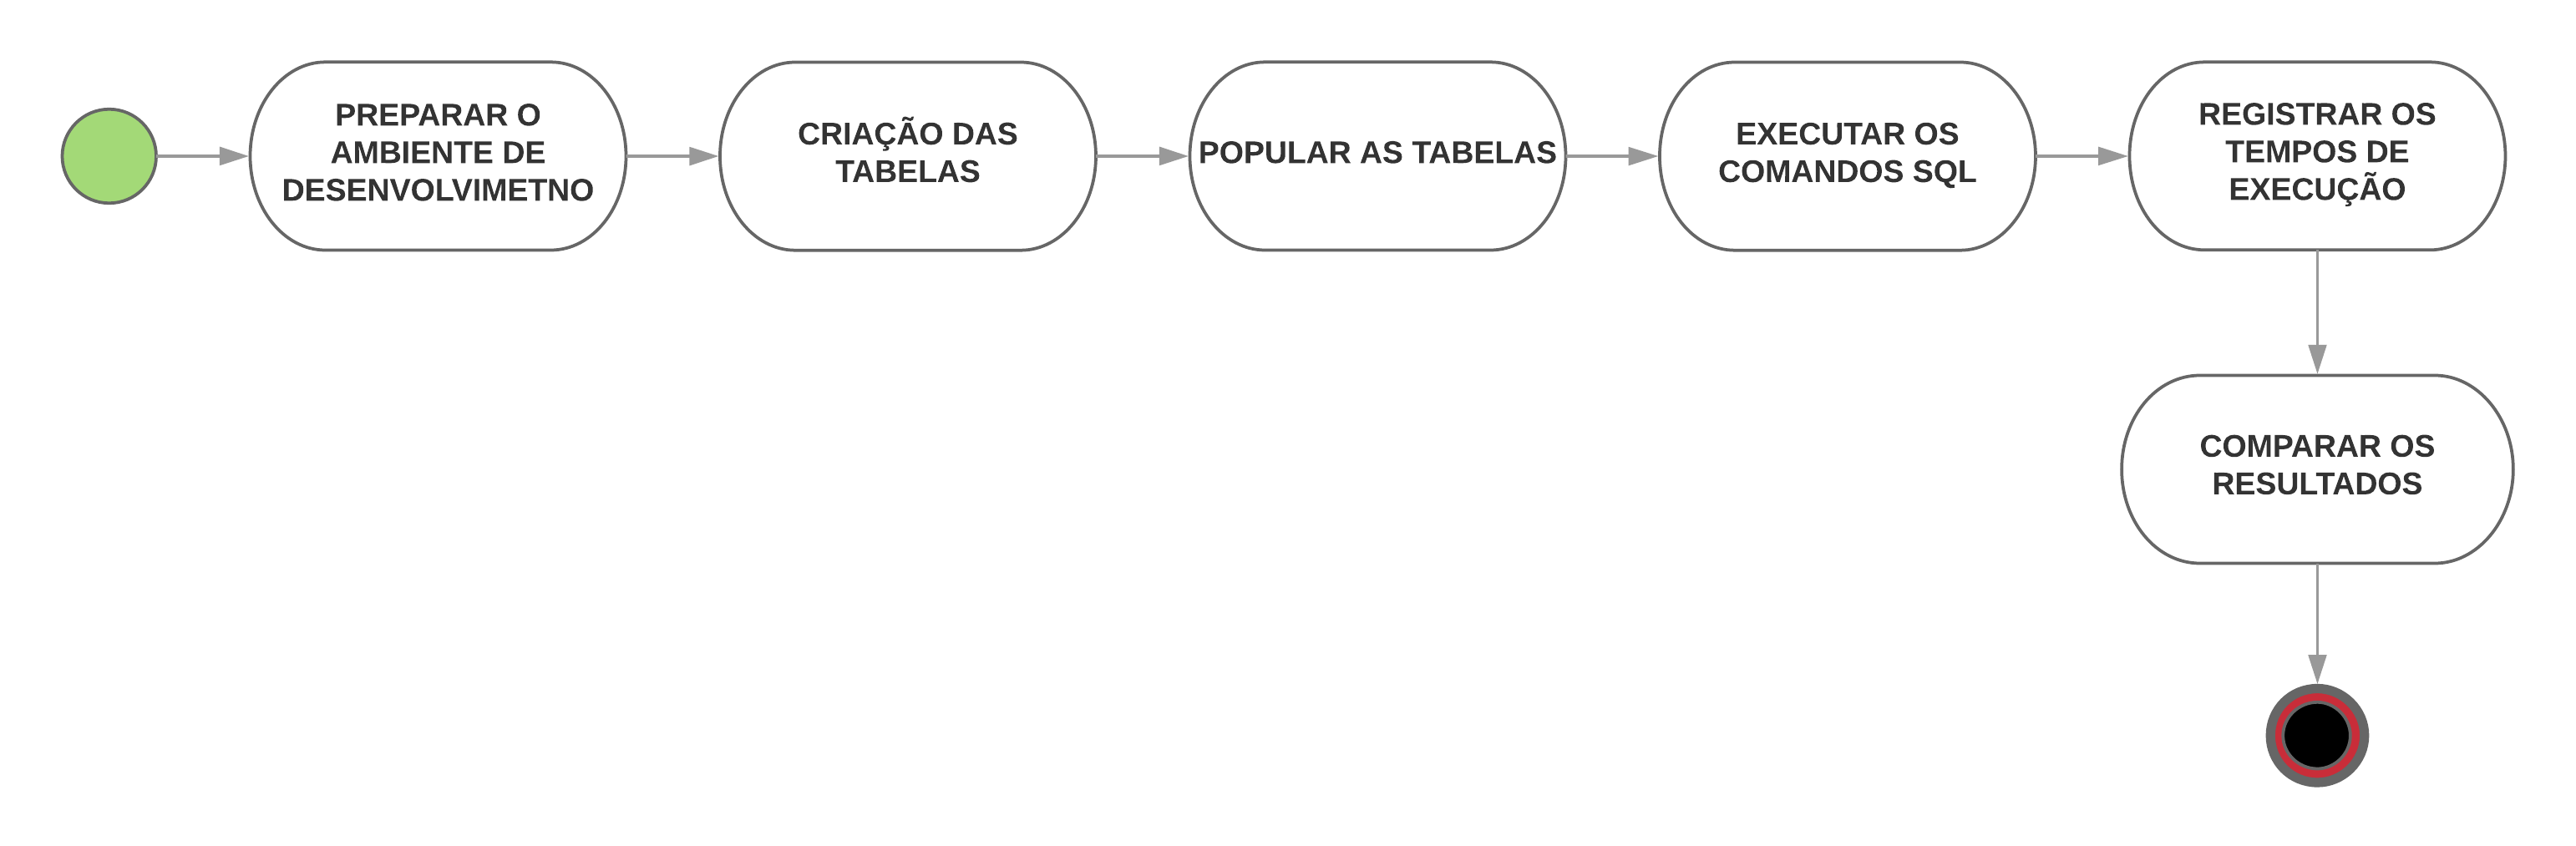
\includegraphics[width=.75\textwidth]{imagem/FLUXO_DEV.png}
%  % Caption centralizada
%  \captionsetup{justification=centering}
%  \captionfont{\small{\textbf{\\Fonte: Autor }}}	
%  \label{fig:4}
%\end{figure}




Como o intuito deste trabalho é realizar alguns testes de performance, entre o banco de dados do SAP ECC e o banco de dados do SAP Hana, realizando algumas consultas de diferentes níveis de dificuldade, atualizações e remoções de dados com o objetivo de medir o tempo de resposta destes SGBDs, se faz necessário detalhar como será o ambiente de testes, o sistema operacional utilizado, hardware e dificuldades encontradas. 

O dados do servidos utilizado estão descritos na tabela 1.
\begin{table}[H]
\centering
\caption{Detalhes do Servidor}
\label{DetalhesServidor}
\begin{tabular}{|l|l|}
\hline
Item                    & Configuração                                                                           \\ \hline
Processador             & Intel(R) Xeon(R) CPU E5-2430 v2 @ 2.50GHz, 2494 Mhz, \\ & 
						  2 Core(s), 2 Logical Processor(s) \\ \hline
Memória RAM             & 8Gb                                                                                    \\ \hline
Disco Rígido            & 150Gb – Disco SATA 10.000   RPM                                                        \\ \hline
Sistema Operacional     & Windows 2008 R2 Standard.                                                              \\ \hline
Banco de dados SAP ECC  & SQL SERVER 2008 R2                                                                     \\ \hline
Banco de dados SAP Hana &                                                                                        \\ \hline
\end{tabular}
\end{table}



%  Este documento foi compilado em ambiente linux (Ubuntu 10.04) usando o programa Kile - an Integrated LaTeX Environment - Version 2.0.85.
%  Para correta formatação os seguintes arquivos do pacote \textit{abntex} devem ser alterados.

 %   \begin{compactitem}
 %     \item[a)] Arquivo abnt.cls

%      No Ubuntu o arquivo fica armazenado em \textit{/usr/share/texmf/tex/latex/abntex}.
%      Comentar a linha 967: Linha comentada para reduzir o espaçamento entre o topo da página e o título.
 %     Alterar a linha 1143: Parâmetro alterado de 30pt para -30pt para reduzir o espaçamento entre o top da página e o título do apêndice.
%      Alterar a linha 985: Parâmetro alterado de 0pt para -30pt para reduzir o espaçamento entre o top da página e o título.
%      Alterar a linha 991: Parâmetro alterado de 45pt para 30pt para reduzir o espaçamento entre o texto e o título.

%      \item[b)] Arquivo acronym.sty

%      No Ubuntu o arquivo fica armazenado em \textit{/usr/share/texmf-texlive/tex/latex/acronym}.
 %     Alterar a linha 225: Inserir o separador -- entre acrônimo/descrição e remover o negrito com o \textit{normalfont}.
      %\item[\protect\AC@hypertarget{#1}{\acsfont{\normalfont{#2}}} --] #3 

 %   \end{compactitem}
% Nome do capítulo
\chapter{Desenvolvimento}
% Label para referenciar
\label{cap4}

% Diminuir espaçamento entre título e texto
\vspace{-1.9cm}

% Texto do capítulo
















%  Este documento foi compilado em ambiente linux (Ubuntu 10.04) usando o programa Kile - an Integrated LaTeX Environment - Version 2.0.85.
%  Para correta formatação os seguintes arquivos do pacote \textit{abntex} devem ser alterados.

 %   \begin{compactitem}
 %     \item[a)] Arquivo abnt.cls

%      No Ubuntu o arquivo fica armazenado em \textit{/usr/share/texmf/tex/latex/abntex}.
%      Comentar a linha 967: Linha comentada para reduzir o espaçamento entre o topo da página e o título.
 %     Alterar a linha 1143: Parâmetro alterado de 30pt para -30pt para reduzir o espaçamento entre o top da página e o título do apêndice.
%      Alterar a linha 985: Parâmetro alterado de 0pt para -30pt para reduzir o espaçamento entre o top da página e o título.
%      Alterar a linha 991: Parâmetro alterado de 45pt para 30pt para reduzir o espaçamento entre o texto e o título.

%      \item[b)] Arquivo acronym.sty

%      No Ubuntu o arquivo fica armazenado em \textit{/usr/share/texmf-texlive/tex/latex/acronym}.
 %     Alterar a linha 225: Inserir o separador -- entre acrônimo/descrição e remover o negrito com o \textit{normalfont}.
      %\item[\protect\AC@hypertarget{#1}{\acsfont{\normalfont{#2}}} --] #3 

 %   \end{compactitem}
 

% Nome do capítulo
\chapter{Testes e Resultados}
% Label para referenciar
\label{cap5}

% Diminuir espaçamento entre título e texto
\vspace{-1.9cm}

% Texto do capítulo
%Para os testes foi simulado valores para cada um dos tipos de pés e pisadas. 

%\begin{figure}[H]
  % Alterar espaçamentos antes e depois do caption
%  \setlength{\abovecaptionskip}{0pt}
%  \setlength{\belowcaptionskip}{0pt}
%  % Caption
%  \caption[Pressão por sensor]{Pressão por sensor}
%  \centering
%  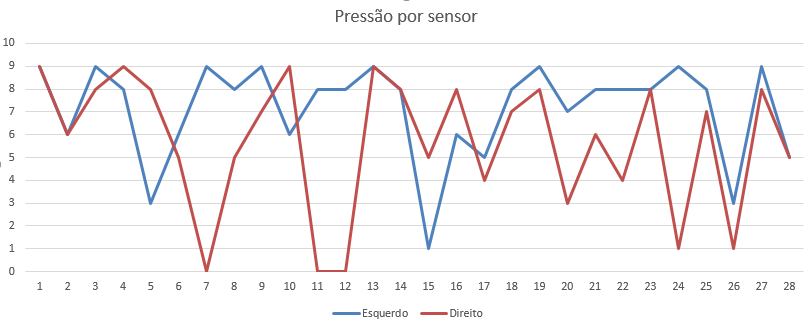
\includegraphics[width=.85\textwidth]{imagem/pressaoporsensor2.png}
  % Caption centralizada
%  \captionsetup{justification=centering}
%  \captionfont{\small{\textbf{\\Fonte: (DEVMEDIA, 2016) }}}	
%  \label{fig:UC}
%\end{figure}

%  Este documento foi compilado em ambiente linux (Ubuntu 10.04) usando o programa Kile - an Integrated LaTeX Environment - Version 2.0.85.
%  Para correta formatação os seguintes arquivos do pacote \textit{abntex} devem ser alterados.

 %   \begin{compactitem}
 %     \item[a)] Arquivo abnt.cls

%      No Ubuntu o arquivo fica armazenado em \textit{/usr/share/texmf/tex/latex/abntex}.
%      Comentar a linha 967: Linha comentada para reduzir o espaçamento entre o topo da página e o título.
 %     Alterar a linha 1143: Parâmetro alterado de 30pt para -30pt para reduzir o espaçamento entre o top da página e o título do apêndice.
%      Alterar a linha 985: Parâmetro alterado de 0pt para -30pt para reduzir o espaçamento entre o top da página e o título.
%      Alterar a linha 991: Parâmetro alterado de 45pt para 30pt para reduzir o espaçamento entre o texto e o título.

%      \item[b)] Arquivo acronym.sty

%      No Ubuntu o arquivo fica armazenado em \textit{/usr/share/texmf-texlive/tex/latex/acronym}.
 %     Alterar a linha 225: Inserir o separador -- entre acrônimo/descrição e remover o negrito com o \textit{normalfont}.
      %\item[\protect\AC@hypertarget{#1}{\acsfont{\normalfont{#2}}} --] #3 

 %   \end{compactitem}
 
% \begin{figure}[H]
  % Alterar espaçamentos antes e depois do caption
%  \setlength{\abovecaptionskip}{0pt}
%  \setlength{\belowcaptionskip}{0pt}
%  % Caption
%  \caption[Cronograma]{Cronograma}
%  \centering
%  \includegraphics[width=.99\textwidth]{imagem/Crono.png}
%  % Caption centralizada
%  \captionsetup{justification=centering}
%  \captionfont{\small{\textbf{\\Fonte: Elaborado pelo autor }}}	
%  \label{fig:UC}
%\end{figure}
% PÓS-TEXTUAIS %%
% Bibliografia no arquivo 'Dissertacao.bib'
% Alterar o título das referências para somente 'Referências'
\renewcommand{\bibname}{Referências}
%\bibliographystyle{abnt-alf}
\bibliography{Dissertacao.bib}

% Para forçar que os apêndices e anexos comecem no anverso
%\setboolean{@openright}{true}

%\apendice
%\begin{apendice}
%%------------------------------------------------------------------------------------------------------------------------------------------------------
% Reiniciar numeração das figuras que aparecem no apêndice
%\setcounter{figure}{0}

%\chapter{Primeiro apêndice}
%\label{apend:codigoMpe}

% Para diminuir espaçamento entre o título e o texto
%\vspace{-1.9cm}

%Textos ou documentos elaborados pelo autor, como por exemplo código-fonte.


%\lstinputlisting[language=C, label=codigo, caption={Trecho de código modificado}]%{pos-texto/codigo.c}
%\end{apendice}

%\anexo
%% Nome do Anexo
%\chapter{Primeiro Anexo}

% Para diminuir espa�amento entre o t�tulo e o texto
%\vspace{-1.9cm}

% Texto
%Textos ou documentos não elaborados pelo autor.

\end{document}